

\documentclass[8pt]{beamer}
\usetheme{default}
\PassOptionsToPackage{usenames,dvipsnames}{xcolor}
\usepackage{my_pres}
\usepackage{tikz}
\usepackage{empheq,accents}
\usepackage{pifont}
\usetikzlibrary{arrows}



% Created by S. Boyd and L. Vandenberghe 
% some traditional definitions that can be blamed on craig barratt
\newcommand{\BEAS}{\begin{eqnarray*}}
\newcommand{\EEAS}{\end{eqnarray*}}
\newcommand{\BEA}{\begin{eqnarray}}
\newcommand{\EEA}{\end{eqnarray}}
\newcommand{\BEQ}{\begin{equation}}
\newcommand{\EEQ}{\end{equation}}
\newcommand{\BIT}{\begin{itemize}}
\newcommand{\EIT}{\end{itemize}}

% text abbrevs
\newcommand{\eg}{{\it e.g.}}
\newcommand{\ie}{{\it i.e.}}

% std math stuff
\newcommand{\ones}{\mathbf 1}
\newcommand{\reals}{{\mbox{\bf R}}}
\newcommand{\integers}{{\mbox{\bf Z}}}
\newcommand{\complex}{{\mbox{\bf C}}}
\newcommand{\symm}{{\mbox{\bf S}}}  % symmetric matrices

% lin alg stuff
\newcommand{\Span}{\mbox{\textrm{span}}}
\newcommand{\range}{{\mathcal R}}
\newcommand{\nullspace}{{\mathcal N}}
\newcommand{\Rank}{\mathop{\bf rank}}
\newcommand{\Tr}{\mathop{\bf tr}}
\newcommand{\cond}{\mathop{\bf cond}}
\newcommand{\diag}{\mathop{\bf diag}}
\newcommand{\lambdamax}{\lambda_{\rm max}}
\newcommand{\lambdamin}{\lambda_{\rm min}}

% probability stuff
\newcommand{\Prob}{\mathop{\bf prob}}
\newcommand{\Expect}{\mathop{\bf E{}}}
\newcommand{\var}{\mathop{\bf var}} % variance
% not sure why we have \Expect and \Prob but \var ???

% convexity & optimization stuff
\newcommand{\Co}{\mathop {\bf conv}} % convex hull
\newcommand{\argmin}{\mathop{\rm argmin}}
\newcommand{\argmax}{\mathop{\rm argmax}}
\newcommand{\epi}{\mathop{\bf epi}}
%\newcommand{\hypo}{\mathop{\bf hypo}}

% sup and inf that look OK in saddle-point form!
%\newcommand{\ourinf}{\mathop{\raisebox{0ex}[0ex][.4ex]{\,inf\,}}}
%\newcommand{\oursup}{\mathop{\raisebox{0ex}[0ex][.4ex]{\,sup\,}}}
\newcommand{\ourinf}{\mathop{\,\mathrm{inf}\, {\rule[-.5ex]{0ex}{0ex}}}}
\newcommand{\oursup}{\mathop{\,\mathrm{sup}\, {\rule[-.5ex]{0ex}{0ex}}}}
%makes latex believe that inf and sup both extend .4ex below
%the baseline

\newcommand{\dist}{\mathop{\bf dist}}
\newcommand{\vol}{\mathop{\bf vol}} % volume
\newcommand{\Card}{\mathop{\bf card}} % cardinality
\newcommand{\sign}{\mathop{\bf sign}}

\newcommand{\dom}{\mathop{\bf dom}} % domain
\newcommand{\aff}{\mathop{\bf aff}} % affine hull
\newcommand{\cl}{\mathop{\bf cl}} % closure
\newcommand{\intr}{\mathop{\bf int}} % interior
\newcommand{\relint}{\mathop{\bf rel int}} % relative interior
\newcommand{\bd}{\mathop{\bf bd}} % boundary

%why do we have the following but not \nust?
\newcommand{\xst}{x^\star}
\newcommand{\lambdast}{\lambda^\star}

% defs for cones & generalized inequalities
% these seem kind of awkward; should fix some day
% rewrite them to use args?
\newcommand{\geqK}{\mathrel{\succeq_K}}
\newcommand{\gK}{\mathrel{\succ_K}}
\newcommand{\leqK}{\mathrel{\preceq_K}}
\newcommand{\lK}{\mathrel{\prec_K}}
\newcommand{\geqKst}{\mathrel{\succeq_{K^*}}}
\newcommand{\gKst}{\mathrel{\succ_{K^*}}}
\newcommand{\leqKst}{\mathrel{\preceq_{K^*}}}
\newcommand{\lKst}{\mathrel{\prec_{K^*}}}
\newcommand{\geqL}{\mathrel{\succeq_L}}
\newcommand{\gL}{\mathrel{\succ_L}}
\newcommand{\leqL}{\mathrel{\preceq_L}}
\newcommand{\lL}{\mathrel{\prec_L}}
\newcommand{\geqLst}{\mathrel{\succeq_{L^*}}}
\newcommand{\gLst}{\mathrel{\succ_{L^*}}}
\newcommand{\leqLst}{\mathrel{\preceq_{L^*}}}
\newcommand{\lLst}{\mathrel{\prec_{L^*}}}

%\newcounter{lecture}
%\newcommand{\lecturefl}[1]{   % use with foiltex landscape
%% \addtocounter{lecture}{1}
% \refstepcounter{lecture}
% \setcounter{equation}{0}
% \setcounter{page}{1}
% \renewcommand{\theequation}{\arabic{equation}}
% \renewcommand{\thepage}{\arabic{lecture}--\arabic{page}}
% \raggedright
% \parindent 0pt
% \rightfooter{\thepage}
% \leftheader{}
% \rightheader{}
% \LogoOff
% \input header 
% \begin{center}
%% {\Large \bfseries Lecture \arabic{lecture} \\*[\bigskipamount] {#1}}
%{\Large \bfseries \arabic{lecture}.  {#1}}
% \end{center}
% \MyLogo{#1}
%}

%\newcommand{\lectureflstar}[1]{   % use with foiltex landscape
% \setcounter{equation}{0}
% \setcounter{page}{1}
% \renewcommand{\theequation}{\arabic{equation}}
% \renewcommand{\thepage}{\arabic{page}}
% \raggedright
% \parindent 0pt
% \rightfooter{\thepage}
% \leftheader{}
% \rightheader{}
% \LogoOff
% \input header 
% \begin{center}
% {\Large \bfseries #1}
% \end{center}
% \MyLogo{#1}
%}
%\newcounter{oursection}
%\newcommand{\frametitle}[1]{  % for use with foiltex landscape
% \addtocounter{oursection}{1}
%% \setcounter{equation}{0}
% \foilhead[-1.0cm]{#1}
% \LogoOn
%}

\newenvironment{algdesc}%
   {\begin{list}{}{%
    \setlength{\rightmargin}{0\linewidth}%
    \setlength{\leftmargin}{.05\linewidth}}%
    \sffamily\small
    \item[]{\setlength{\parskip}{0ex}\hrulefill\par%
    \nopagebreak{}}}%
   {{\setlength{\parskip}{-1ex}\nopagebreak\par\hrulefill} \end{list}}

\newenvironment{colm}{\left[\begin{array}{c}}{\end{array}\right]}
\newenvironment{colv}{\left(\begin{array}{c}}{\end{array}\right)}




\definecolor{texthigh}{RGB}{137, 0, 255}
\definecolor{textred}{RGB}{255, 0, 94}
\definecolor{textgreen}{RGB}{89, 232, 151}
\definecolor{textlightgray}{RGB}{170,170,170}
\definecolor{bggray}{RGB}{230,230,230}
\definecolor{textgray}{RGB}{60,60,60}

\setbeamercolor{background canvas}{bg=bggray}
\setbeamercolor{normal text}{fg=textgray}

\setbeamertemplate{enumerate items}[default]
\setbeamertemplate{itemize items}{\ding{84}}

\title{Improving Multiset Canonical Correlation Analysis in High Dimensional Sample
  Deficient Settings}
\institute[Univ. of Michigan]{Department of Electrical Engineering and Computer
  Science\\University of Michigan\\ }
\author[N. Asendorf, R.R. Nadakuditi]{Nicholas Asendorf, Ph.D. \hspace{10ex} Prof. Raj
  Nadakuditi\\ {\small{\texttt{asendorf@umich.edu} \phantom{addk}\hspace{12ex}
      \texttt{rajnrao@umich.edu}}  }}
\date{Asilomar Conference on Signals, Systems, and Computers\\[2ex] November 9, 2015}

\newcommand{\twr}{{\sf TW}_\reals}
\newcommand{\twc}{{\sf TW}_\complex}
\newcommand{\sx}{s_{x,i}}
\newcommand{\sy}{s_{y,i}}
\newcommand{\zx}{z_{x,i}}
\newcommand{\zy}{z_{y,i}}
\newcommand{\Zx}{Z_x}
\newcommand{\Zy}{Z_y}
\newcommand{\Ux}{U_x}
\newcommand{\Uy}{U_y}
\newcommand{\Vx}{V_x}
\newcommand{\Vy}{V_y}
\newcommand{\Pxy}{P_{xy}}
\newcommand{\kx}{k_x}
\newcommand{\ky}{k_y}
\newcommand{\kxhat}{\widehat{k}_x}
\newcommand{\kyhat}{\widehat{k}_y}
\newcommand{\khatcca}{\widehat{k}_{\text{cca}}}
\newcommand{\khaticca}{\widehat{k}_{\text{icca}}}
\newcommand{\Uxhat}{\widehat{U}_x}
\newcommand{\Uyhat}{\widehat{U}_y}
\newcommand{\Sigxhat}{\widehat{\Sigma}_x}
\newcommand{\Sigyhat}{\widehat{\Sigma}_y}
\newcommand{\Vxhat}{\widehat{V}_x}
\newcommand{\Vyhat}{\widehat{V}_y}
\newcommand{\Uxtil}{\widetilde{U}_x}
\newcommand{\Uytil}{\widetilde{U}_y}
\newcommand{\Vxtil}{\widetilde{V}_x}
\newcommand{\Vytil}{\widetilde{V}_y}
\newcommand{\Uxcir}{\accentset{\circ}{U}_x}
\newcommand{\Ukcir}{\accentset{\circ}{U}_{\widetilde{K}}}
\newcommand{\Uycir}{\accentset{\circ}{U}_y}
\newcommand{\Sigxcir}{\accentset{\circ}{\Sigma}_x}
\newcommand{\Sigycir}{\accentset{\circ}{\Sigma}_y}
\newcommand{\Vxcir}{\accentset{\circ}{V}_x}
\newcommand{\Vycir}{\accentset{\circ}{V}_y}
\newcommand{\kapcir}{\accentset{\circ}{\kappa}}
\newcommand{\xii}{x_i}
\newcommand{\yii}{y_i}
\newcommand{\Tx}{\Theta_x}
\newcommand{\Ty}{\Theta_y}
\newcommand{\Txhat}{\widehat{\Theta}_x}
\newcommand{\Tyhat}{\widehat{\Theta}_y}
\newcommand{\tx}{\theta^{(x)}}
\newcommand{\ty}{\theta^{(y)}}
\newcommand{\Kxy}{K_{xy}}
\newcommand{\Kxytil}{\widetilde{K}_{xy}}
\newcommand{\Uktil}{U_{\widetilde{K}}}
\newcommand{\Vktil}{V_{\widetilde{K}}}
\newcommand{\Uktilhat}{\widehat{U}_{\widetilde{K}}}
\newcommand{\Vktilhat}{\widehat{V}_{\widetilde{K}}}
\newcommand{\kxy}{k^{xy}}
\newcommand{\defeq}{=:}
\newcommand{\Rxx}{R_{xx}}
\newcommand{\Ryy}{R_{yy}}
\newcommand{\Rxy}{R_{xy}}
\newcommand{\Rxxhat}{\widehat{R}_{xx}}
\newcommand{\Ryyhat}{\widehat{R}_{yy}}
\newcommand{\Rxyhat}{\widehat{R}_{xy}}
\newcommand{\wx}{w_x}
\newcommand{\wy}{w_y}
\newcommand{\wxt}{\widetilde{w}_x}
\newcommand{\wyt}{\widetilde{w}_y}
\newcommand{\wxicca}{\widehat{w}_x^{\text{icca}}}
\newcommand{\wyicca}{\widehat{w}_y^{\text{icca}}}
\newcommand{\wxticca}{\widetilde{w}_x^{\text{icca}}}
\newcommand{\wyticca}{\widetilde{w}_y^{\text{icca}}}
\newcommand{\wxhaticca}{\widehat{w}_x}
\newcommand{\wyhaticca}{\widehat{w}_y}
\newcommand{\Ccca}{C_{\text{cca}}}
\newcommand{\Cccahat}{\widehat{C}_{\text{cca}}}
\newcommand{\Ciccahat}{\widehat{C}_{\text{icca}}}
\newcommand{\Ciccat}{\widetilde{C}_{\text{icca}}}
\newcommand{\rank}{\text{rank}}
\newcommand{\taucca}{\tau_{\text{cca}}^\alpha}
\newcommand{\tauicca}{\tau_{\text{icca}}^\alpha}
\newcommand{\simiid}{\overset{\text{i.i.d.}}{\sim}}
\newcommand{\rhocca}{\rho_\text{cca}}
\newcommand{\rhohatcca}{\widehat{\rho}_\text{cca}}
\newcommand{\rhohaticca}{\widehat{\rho}_\text{icca}}
\newcommand{\rhoeff}{k_{\text{eff}}^{xy}}
\newcommand{\Cmcca}{C_{\text{mcca}}}
\newcommand{\Ucir}{\accentset{\circ}{U}}
\newcommand{\Vcir}{\accentset{\circ}{V}}
\newcommand{\Cmccatil}{\widetilde{C}_{\text{mcca}}}

\newcommand{\iccap}{ICCA\texttt{+} }
\newcommand{\iccaps}{ICCA\texttt{+}}
\newcommand{\Sigxtil}{\widetilde{\Sigma}_x}
\newcommand{\Sigytil}{\widetilde{\Sigma}_y}

\newcommand{\Cmccahat}{\widehat{C}_{\text{mcca}}}
\newcommand{\Cimccahat}{\widehat{C}_{\text{imcca}}}

%\newcommand{\kapcir}{\accentset{\circ}{\kappa}}
%\newcommand{\simiid}{\overset{\text{i.i.d.}}{\sim}}
%\newcommand{\twc}{{\sf TW}_\complex}

%\newcommand{\Uxcir}{\accentset{\circ}{U}_x}
%\newcommand{\Uycir}{\accentset{\circ}{U}_y}
%\newcommand{\Vxcir}{\accentset{\circ}{V}_x}
%\newcommand{\Vycir}{\accentset{\circ}{V}_y}

\begin{document}

%--- the titlepage frame -------------------------%
\begin{frame}[plain]
  \titlepage
  \addtocounter{framenumber}{-1}
\end{frame}


%%%%%%%%%%%%%%%%%%%%%%%%%%%%%%%%%%%%%%%%%%%%%%%%%%%%%%%%%%%%%%%%%%%%%%
\begin{frame}{Motivation}

  \begin{center}
    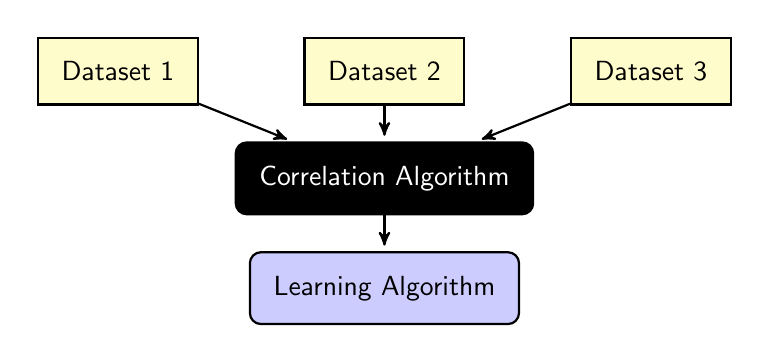
\begin{tikzpicture}[
      font=\sffamily,
      every matrix/.style={ampersand replacement=\&,column sep=3ex,row sep=3ex},
      dataset/.style={draw,thick,fill=yellow!20,inner sep=.3cm},
      sink/.style={dataset,rounded corners,fill=black, text=white},
      app/.style={dataset,rounded corners,fill=blue!20},
      dots/.style={gray,scale=2},
      to/.style={->,>=stealth',shorten >=2pt,thick,font=\sffamily\footnotesize},
      every node/.style={align=center}]

      \matrix{
        \node[dataset] (dataset1) {Dataset 1};
        \& \node[dataset] (dataset2) {Dataset 2};
        \& \node[dataset] (dataset3) {Dataset 3}; \\

        \& \node[sink] (blackbox) {Correlation Algorithm}; \& \\

        \& \node[app] (application) {Learning Algorithm}; \& \\      
      };

      \draw[to] (dataset1) -- (blackbox);
      \draw[to] (dataset2) -- (blackbox);
      \draw[to] (dataset3) -- (blackbox);
      \draw[to] (blackbox) -- (application);

    \end{tikzpicture}
  \end{center}

  \begin{center}
    \textbf{Goal}\\
    \vspace{1ex}
    \fcolorbox{black}[HTML]{F1F1F1}{\parbox{0.6\textwidth}{%
        \centering Develop theoretically justified, robust\\ correlation algorithms for\\
        multi-dataset fusion}}
  \end{center}

    
\end{frame}

\begin{frame}{A Myriad of Applications}

  \begin{columns}[T]
    \begin{column}{0.45\textwidth}
      
      \vspace{3ex}

      \textbf{Multiple Datasets}
      \begin{itemize}
      \item \textcolor<1>{texthigh}{Audio-Video}
      \item \textcolor<2>{texthigh}{Audio-Audio}
      \end{itemize}

      \hspace{2ex}
      

      \textbf{Machine Learning}
      \begin{itemize}
      \item \textcolor<3>{texthigh}{emotion identification}
      \item \textcolor<4>{texthigh}{shopping predictions}
      \item \textcolor<5>{texthigh}{music genre classification}
      \end{itemize}
      
      \hspace{2ex}

      \textbf{Medical Signal Processing}
      \begin{itemize}
      \item MRI, fMRi, EEG, MEG, etc.
      \end{itemize}


    \end{column}
    \begin{column}{0.45\textwidth}
      \begin{center}
      \includegraphics<1>[width=0.6\textwidth]{figures/parking_lot.jpg}\vspace{3ex}
      \includegraphics<1>[width=0.6\textwidth]{figures/car.png}
      \includegraphics<2>[width=0.8\textwidth]{figures/burton.jpg}
      \includegraphics<3>[width=0.6\textwidth]{figures/emotion1.png}
      \includegraphics<4>[width=0.8\textwidth]{figures/amazon_books.jpg}
      \includegraphics<5>[width=0.8\textwidth]{figures/Queen-Band.jpg}

      \vspace{4ex}

      \includegraphics<1>[width=0.6\textwidth]{figures/parking_lot2.jpg}
      \includegraphics<2>[width=0.8\textwidth]{figures/umich.png}
      \includegraphics<3>[width=0.7\textwidth]{figures/speaker_audio.pdf}
      \includegraphics<4>[width=0.8\textwidth]{figures/amazon_movies.jpg}
      \onslide<5>{\fcolorbox{black}[HTML]{F1F1F1}{\parbox{0.9\textwidth}{%
        \begin{itemize}
        \item disco influences
        \item danceable grooves
        \item repetitive melodic phrasing
        \item extensive vamping
        \item minor key tonality
        \end{itemize}}}}

  \end{center}
    \end{column}
  \end{columns}


\end{frame}


%%%%%%%%%%%%%%%%%%%%%%%%%%%%%%%%%%%%%%%%%%%%%%%%%%%%%%%%%%%%%%%%%%%%%%%
\begin{frame}{MCCA - Multiset Canonical Correlation Analysis}


\textbf{Notation}
\begin{itemize}
\item data: $y_1\in\complex^{d_1\times 1},\dots,y_m\in\complex^{d_m\times 1}$
\item covariance matrices: $R_{ij} = \E{y_iy_j^H}$
\item canonical vectors: $x_1,\dots,x_m$
\item canonical variates: $w_1,\dots, w_m$, $w_i=x_i^Hy_i$
\end{itemize}

\vspace{2ex}

\begin{equation*}
\Phi(x)=E[ww^H]=\left[\begin{array}{ccc} x_1^HR_{11}x_1 & \dots & x_1^HR_{1m}x_m \\ \vdots
    & \ddots & \vdots \\ x_m^HR_{m1}x_1 & \dots & x_m^HR_{mm}x_m\\ \end{array}\right]
\end{equation*}

\vspace{1ex}

\begin{center}
  \textbf{Optimization Problem}\\

  \fcolorbox{black}[HTML]{F1F1F1}{\parbox{0.5\textwidth}{%
      \be\ba
      &\underset{x}{\mathop{\rm optimize}} && J(\Phi(x))\\
      &\mathop{\rm subject~ to} && h(x,R)\\
      \ea\ee
    }}
\end{center}


\end{frame}

%%%%%%%%%%%%%%%%%%%%%%%%%%%%%%%%%%%%%%%%%%%%%%%%%%%%%%%%%%%%%%%%%%%%%%%
\begin{frame}{MCCA - Multiset Canonical Correlation Analysis}

  \addtocounter{framenumber}{-1}
\textbf{Notation}
\begin{itemize}
\item data: $y_1\in\complex^{d_1\times 1},\dots,y_m\in\complex^{d_m\times 1}$
\item covariance matrices: $R_{ij} = \E{y_iy_j^H}$
\item canonical vectors: $x_1,\dots,x_m$
\item canonical variates: $w_1,\dots, w_m$, $w_i=x_i^Hy_i$
\end{itemize}

\vspace{2ex}

\begin{equation*}
\Phi(x)=E[ww^H]=\left[\begin{array}{ccc} x_1^HR_{11}x_1 & \dots & x_1^HR_{1m}x_m \\ \vdots
    & \ddots & \vdots \\ x_m^HR_{m1}x_1 & \dots & x_m^HR_{mm}x_m\\ \end{array}\right]
\end{equation*}

\vspace{1ex}

  \begin{center}
    \textbf{MAXVAR Optimization Problem}\\
    \fcolorbox{black}[HTML]{F1F1F1}{\parbox{0.4\textwidth}{%
        \be\ba
        &\argmax_{x_1,\dots,x_m}&&\rho_{\text{mcca}}=\lambda_1\left(\Phi(x)\right)\\
        &\text{subject to} &&x_i^HR_{ii}x_i = 1
        \ea\ee
      }}
  \end{center}

\end{frame}

%%%%%%%%%%%%%%%%%%%%%%%%%%%%%%%%%%%%%%%%%%%%%%%%%%%
\begin{frame}{MCCA Solution and Empirical Solution}

  \begin{columns}
    \begin{column}{0.5\textwidth}
      \textbf{Notation}
      \begin{itemize}
      \item $R = \left[R_{ij}\right]_{i,j=1}^m$
      \item $R_D = \blkdiag(R_{11},\dots,R_{mm})$
      \item $C_{\text{mcca}}= R_D^{-/12}RR_D^{-1/2}$
      \end{itemize}
    \end{column}
    \begin{column}{0.5\textwidth}
        \begin{center}
    \textbf{MCCA Solution}\\
    \fcolorbox{black}[HTML]{F1F1F1}{\parbox{0.8\textwidth}{%
        \be
        \rho^{(j)}_{\text{mcca}} = \lambda_j\left(C_{\text{mcca}}\right)
        \ee
      }}
  \end{center}

    \end{column}
  \end{columns}

  \vspace{5ex}

  \pause

  \textbf{Empirical MAXVAR}
  \begin{itemize}
  \item Covariance matrices $R_{ij}$ are typically unknown in practice
  \item Training data $Y_j=\left[y_1^{(j)},\dots,y_n^{(j)}\right]$, $j=1,\dots,m$
  \item Sample covariance matrices $\widehat{R}_{ij}= \frac{1}{n}Y_iY_j^H$
  \item Form $\widehat{R}$ and $\widehat{R}_D$
  \item $\widehat{C}_\text{mcca} = \widehat{R}_D^{-/12}\widehat{R}\widehat{R}_D^{-1/2}$
  \end{itemize}

  \vspace{2ex}

  \begin{center}
    \textbf{Proposed correlation statistic}\\
    \fcolorbox{black}[HTML]{F1F1F1}{\parbox{0.4\textwidth}{%
        \be
        \widehat{\rho}^{(j)}_{\text{mcca}} = \lambda_j\left(\Cmccahat - I\right)
        \ee
      }}
  \end{center}



\end{frame}

%%%%%%%%%%%%%%%%%%%%%%%%%%%%%%%%%%%%%%%%%%%%%
\begin{frame}{Empirical MCCA Insights}


  \textbf{Empirical MAXVAR Equivalency}
  \begin{itemize}
  \item Let $Y_j=\widehat{U}_j\widehat{\Sigma}_j\widehat{V}_j$ be SVD of dataset $j$
  \item Let $\widetilde{U}=\blkdiag(\widehat{U}_1,\dots,\widehat{U}_m)$
  \item Let $\widetilde{V}=[\widehat{V}_1,\dots,\widehat{V}_m]$
  \item $\widehat{C}_{\text{mcca}}=
    \widetilde{U}\widetilde{V}^H\widetilde{V}\widetilde{U}$
  \item $\lambda_j\left(\widehat{C}_{\text{mcca}}\right) =
    \lambda_j\left(\widetilde{V}^H\widetilde{V}\right)$ 
  \end{itemize}

  \vspace{3ex}
  \textbf{Insights}
  \begin{itemize}
  \item This uses \textit{ALL} right singular vectors
  \item In many applications, low-rank setting 
  \item In low-SNR, low-sample regime, singular vectors may be inaccurate
  \item We can use insights from random matrix theory (RMT) to quantify singular vector
    accuracy to improve MCCA
  \item Let $\widehat{k}_j$ be RMT estimates of rank of each dataset
  \end{itemize}

\end{frame}

%%%%%%%%%%%%%%%%%%%%%%%%%%%%%%%%%%%%%%%%%%%%%
\begin{frame}{IMCCA - Informative MCCA}

  \textbf{Idea - Trim right singular vectors}
  \begin{itemize}
  \item  $\Vcir_i = \widehat{V}_i\left(:,1:\widehat{k}_i\right)$
  \item  $\Vcir =\left[\Vcir_1,\dots \Vcir_m\right]$
  \end{itemize}

  \begin{columns}[t]
    \begin{column}{0.5\textwidth}
      \begin{center}
        \textbf{New IMCCA Matrix}\\
        \fcolorbox{black}[HTML]{F1F1F1}{\parbox{0.8\textwidth}{%
            \be
            \Cimccahat = \Vcir^H\Vcir
            \ee
          }}
      \end{center}
    \end{column}
    \begin{column}{0.5\textwidth}
      \begin{center}
        \textbf{Proposed correlation statistic}\\
        \fcolorbox{black}[HTML]{F1F1F1}{\parbox{0.8\textwidth}{%
            \be
            \widehat{\rho}^{(j)}_{\text{imcca}} = \lambda_j\left(\Cimccahat - I\right)
            \ee
          }}
      \end{center}
    \end{column}
  \end{columns}

  \vspace{2ex}

  \textbf{Insights}
  \begin{itemize}
  \item Eigenvalue detects correlation
  \item Eigenvector reveals structure
  \end{itemize}


\end{frame}

%%%%%%%%%%%%%%%%%%%%%%%%%%%%%%%%%%%%
\begin{frame}{Numerical Simulation}

  \begin{itemize}
  \item rank-1 setting, $m=3$, $d_1=d_2=d_3=150$
  \item $y_j^{(i)}=U_js_j^{(i)} + z_j^{(i)}$
  \item $z_j\sim\mathcal{CN}(0,I)$, $s_j^{(i)} \sim \mathcal{CN}(0,\theta)$
  \item $\E{s_js_i} = 0.9$
  \item Plot KS-statistic of $\widehat{\rho}^{(j)}_{\text{mcca}}$ and
    $\widehat{\rho}^{(j)}_{\text{imcca}}$ for signal-plus-noise vs. noise only
  \end{itemize}

  \vspace{2ex}

  \begin{center}
    \hspace{-3ex}\textbf{Empirical MCCA}\hspace{25ex}\textbf{IMCCA}\\
    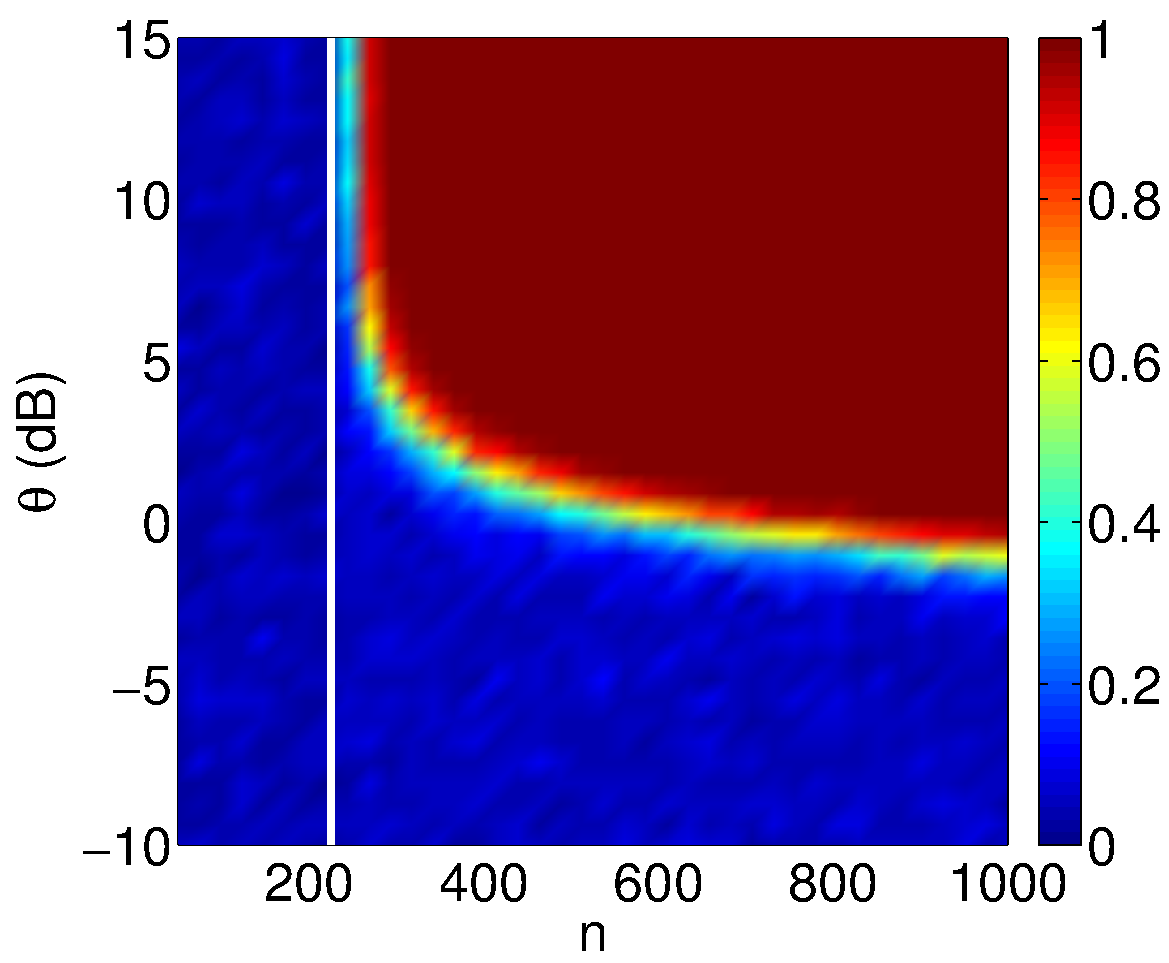
\includegraphics[width=0.45\textwidth]{figures/mcca_pt.pdf}\hspace{2ex}
    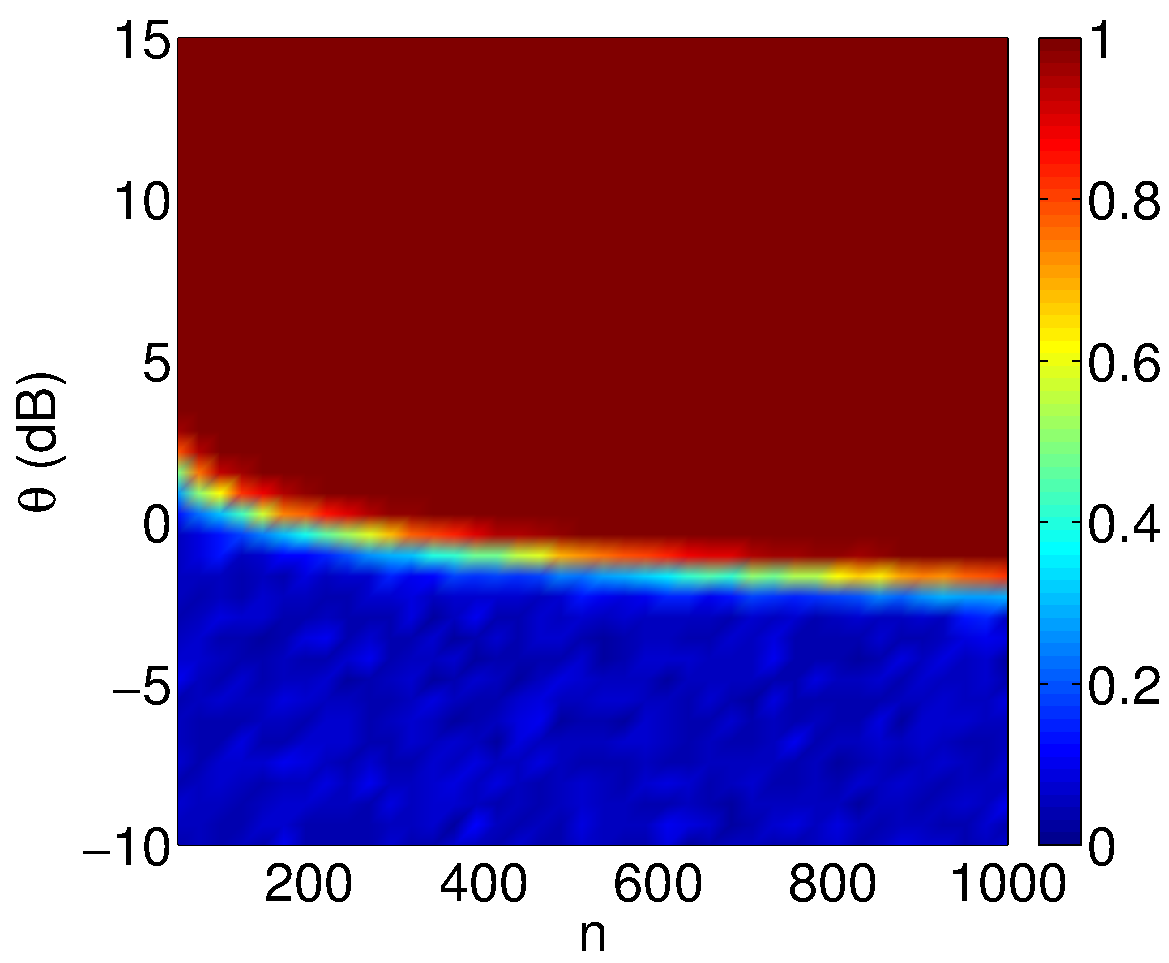
\includegraphics[width=0.45\textwidth]{figures/imcca_pt.pdf}

  \end{center}


\end{frame}

%%%%%%%%%%%%%%%%%%%%%%%%%%%%%%%%%%%%%%%%%%%%%
\begin{frame}{\href{run:/home/asendorf/Documents/thesis_videos/mcca_flashing.mp4}{Empirical
      MCCA and
      IMCCA Demonstration}} 

    \begin{center}
      \hspace{-3ex}\textbf{Empirical MCCA Correlations}\hspace{13ex}\textbf{IMCCA Correlations}
        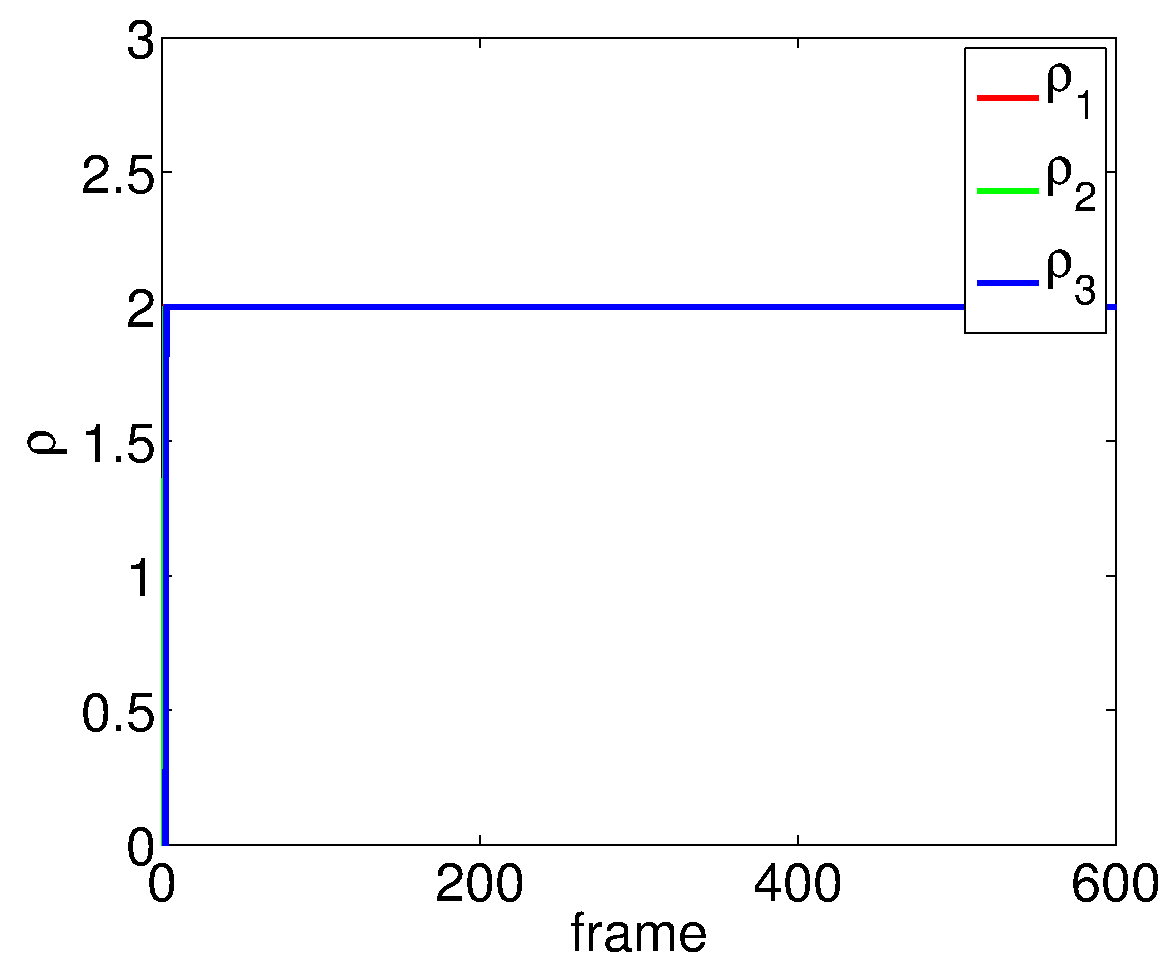
\includegraphics[width=0.45\textwidth]{figures/mcca_cca_corrs.pdf}\hspace{2ex}
        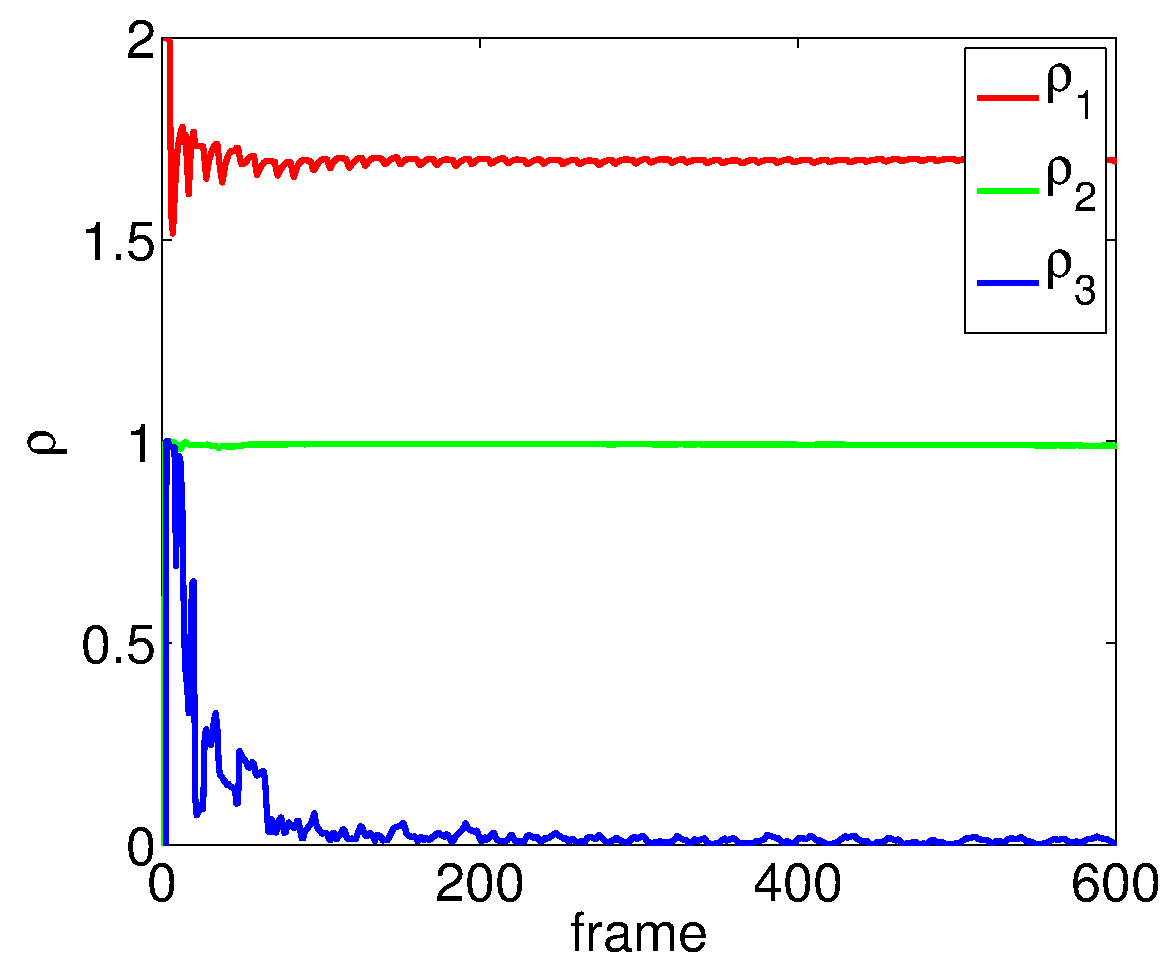
\includegraphics[width=0.45\textwidth]{figures/mcca_icca_corrs.pdf}
    \end{center}

\end{frame}

%%%%%%%%%%%%%%%%%%%%%%%%%%%%%%%%%%%%
\begin{frame}{Conclusion}

  \begin{center}
  \textbf{Take Home Message}\\
  \fcolorbox{black}[HTML]{F1F1F1}{\parbox{0.5\textwidth}{
      \centering
      Trim then fuse \textbf{\textit{ NOT }} fuse then trim
    }}
  \end{center}

  \vspace{3ex}

  \textbf{Contributions}
  \begin{itemize}
  \item Proposed IMCCA algorithm
  \item Proposed statistics to detect latent correlations in more than 2 datasets
  \item Acheived better performance in low-SNR, high dimensional setting 
  \end{itemize}
\end{frame}

\end{document}
